\section{A ground truth from zone price deviations}
\label{sec:zones}

\subsection{Finding the deviations}

Dominick's set regular prices by zone: within a zone every store was meant to
carry the same regular price~\cite{dominicks}. For each store and item we take
the log of the week's regular price (no deal code, not more than 5\% below the
item's highest price in that store over the last 12 weeks) over that item's
median regular price in that store over all weeks, and subtract the median of
the same across the zone's stores that week. Moves made zone-wide cancel, and
so do an item's usual price differences between stores; a store moved on its
own stands out. An episode is at least 12 consecutive weeks in which this
quantity is at least 3\% in the same direction for at least 60\% of the store's
items, with a median of at least 5\% over the episode. Controls are stores of
the same zone within 1\% of their zone over those weeks. An episode with fewer
than three controls is listed but not scored.

The detector was written, and its episodes listed, before any model was scored
against them. A first version measured stores against the zone's most common
price and found one episode, in analgesics: in the experiments a third of a
zone's stores moved up and a third down, so the most common price was often a
moved one. The change is recorded, with its date, in the plan.

\subsection{Measuring their effect}

For episode $e$ of store $s$ with controls $\mathcal C_e$, the response is the
difference in differences on log category units,
\begin{equation}
  \log Y_{jw} = \alpha_j + \gamma_w + \tau_e\, D_{jw} + \varepsilon_{jw},
  \qquad j \in \{s\} \cup \mathcal C_e,
\end{equation}
over the 26 weeks before the episode and its first eight weeks, where $Y_{jw}$
is store $j$'s category units in week $w$ and $D_{jw}$ marks the treated store
in the episode weeks. Standard errors are clustered by
store~\cite{bertrand2004,cameron2015} with the CR1 correction and $t$ critical
values on stores minus one degrees of freedom; with four to eight stores per
episode, single intervals are wide by construction, and the pooled slope of
$\tau_e$ on $\delta_e$ across episodes is the main summary. The estimate over
the full episode is kept in the list as well. The models forecast at most eight
weeks ahead, so each model is fitted on the data up to the week before an
episode and scored on its first eight weeks, the same weeks as $\tau_e$.

\subsection{What the deviations show}

\begin{figure*}[t]
\centering
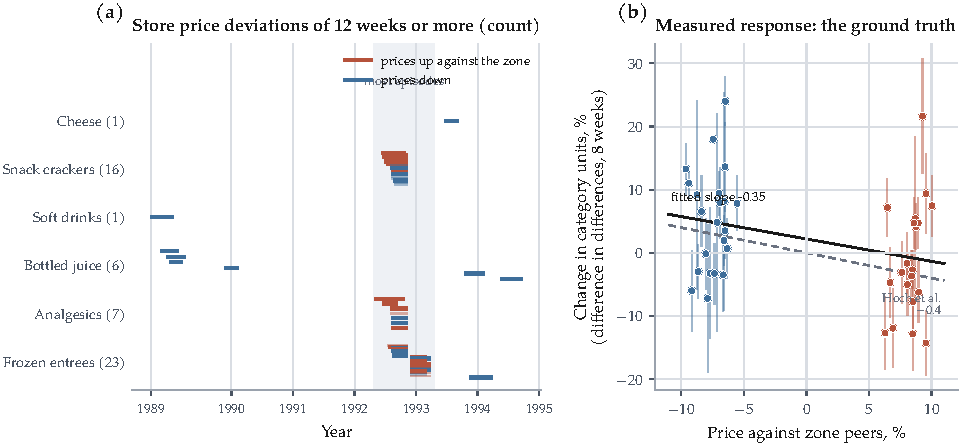
\includegraphics[width=\textwidth]{figs/fig_zones.pdf}
\caption{\textbf{The price deviations cluster in 1992 and 1993, when the chain
ran its pricing experiments, and on average sales move against price.}
\textbf{(a)} Every episode found in the six categories (count in brackets);
faint: fewer than three control stores, listed but not scored. \textbf{(b)} For
the \zScored{} scored episodes, the store's price against its zone peers and
the measured change in its category units over the episode's first 8 weeks
(difference in differences against same-zone stores, store and week fixed
effects, 95\% interval clustered by store; these intervals are too narrow, see
Figure~\ref{fig:zonechecks}). Solid line: fitted slope; dashed: the $-0.4$
elasticity reported for the experiments~\cite{hoch1994}.}
\label{fig:zones}
\end{figure*}

The detector finds \zEpisodes{} episodes in the six categories, \zScored{} with at
least three control stores (Figure~\ref{fig:zones}). Most lie between Dominick's
weeks 190 and 240, mid 1992 to mid 1993, the period of the chain's experiments;
the scored stores' prices sit \zSizeLo\% to \zSizeHi\% off their zone peers.
Over the first eight weeks of each scored episode, category units move against
price in \zSignShare\% of episodes. The pooled slope of the measured response on
the price change is $\zSlope$, with a 95\% interval of $\zSlopeLo$ to
$\zSlopeHi$ (heteroskedasticity-robust across episodes), and over the full
episode $\zFullSlope$ ($\zFullLo$ to $\zFullHi$). Both are in line with the
$-0.4$ Hoch, Dr\`eze and Purk report, and neither is precise.

\begin{figure*}[t]
\centering
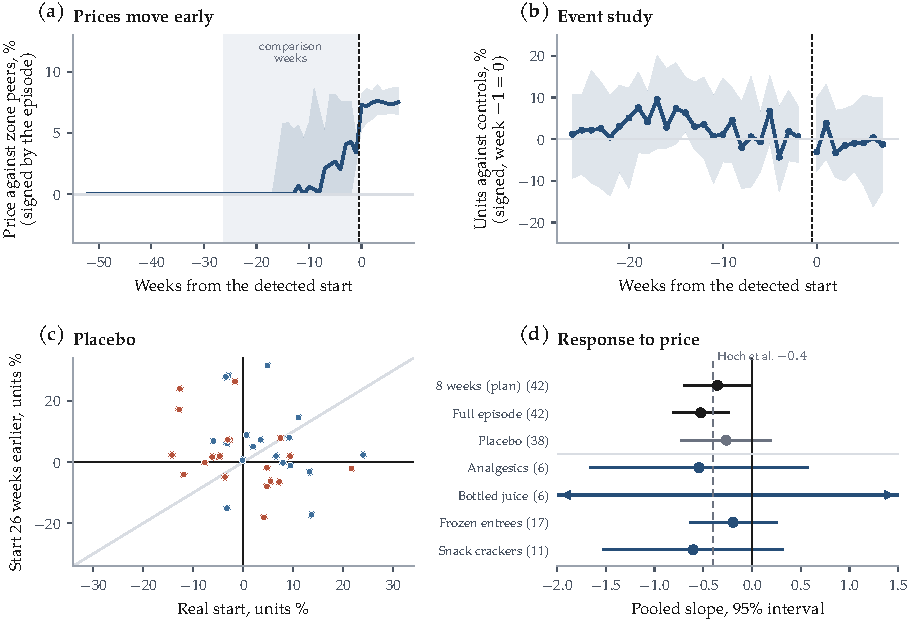
\includegraphics[width=\textwidth]{figs/fig_zone_checks.pdf}
\caption{\textbf{Prices start moving before the detected start, single
episodes are mostly noise, and only the pooled response carries information.}
\textbf{(a)} The store's regular prices against its zone peers, signed by the
episode's direction: median and interquartile band across the \zScored{} scored
episodes; shaded, the 26 comparison weeks of the difference in differences.
\textbf{(b)} Event study: weekly coefficients signed the same way, week $-1$ as
reference; median and interquartile band. \textbf{(c)} The 8-week estimate with
the start moved 26 weeks earlier, where prices had not moved, against the real
estimate; red, prices up; blue, down. \textbf{(d)} Pooled slopes of the
response on the price change with 95\% intervals, for the plan's 8-week
estimate, the full episode, the placebo, and each category with at least five
episodes (count in brackets). The detection rule, controls and estimator were
fixed in advance; panels (a) and (d) were added after the placebo was seen.}
\label{fig:zonechecks}
\end{figure*}

Three robustness analyses, fixed in advance, and two added after seeing them
qualify this ground truth (Figure~\ref{fig:zonechecks}).

\paragraph{Prices move before the detected start}
The detector dates an episode from the first week in which most of the store's
items are at least 3\% off. Prices ease in before that: in the eight weeks before
the detected start, \zEarlyShare\% of store-weeks are already 3\% or more off in
the episode's direction (panel a). Part of the 26 comparison weeks is therefore
treated, which biases the 8-week estimate towards zero and shows in the event
study as a gradual decline in signed sales over the weeks before the start
(panel b). The full-episode estimate, which compares the whole spell, is
larger, $\zFullSlope$ against $\zSlope$.

\paragraph{Single episodes are noise}
Moved 26 weeks earlier, to weeks where prices had not moved, the same estimator
gives a pooled slope of $\zPlaceboSlope$ ($\zPlaceboLo$ to $\zPlaceboHi$), and
\zPlaceboSig\% of the \zPlaceboN{} placebo intervals exclude zero, where 5\%
should. The intervals clustered by store are far too narrow: their median
standard error is \zEpisodeSE{} while placebo estimates spread with a standard
deviation of \zPlaceboSD. With four to eight stores, weekly category sales that
move together over many weeks, and errors clustered by so few
stores, this is the failure Bertrand, Duflo and Mullainathan~\cite{bertrand2004}
and Cameron and Miller~\cite{cameron2015} describe. A single episode's
interval, and with it the plan's per-episode score for C7, cannot be trusted;
the comparison of models with the measured response is made on the pooled
slope and its interval.

\paragraph{The pooled response is stable but imprecise}
Over the nine detector settings (Table~\ref{tab:sensitivity}) the number of
scored episodes ranges from \zSensLo{} to \zSensHi{} and the pooled slope from
$\zSensSlopeLo$ to $\zSensSlopeHi$. By category, the slope is negative in
\zCatNeg{} of the \zCatN{} categories with at least five episodes, and every
category's interval is wide (panel d).

\begin{table}[t]
\centering
\caption{\textbf{The pooled response keeps its sign under every detector
setting.} Episodes found and scored, and the pooled 8-week slope, for each
weekly size and episode median; the plan's setting in bold.}
\label{tab:sensitivity}
\footnotesize
\begin{tabular}{@{}rrrrr@{}}
\toprule
Each week & Episode median & Episodes & Scored & Slope \\
\midrule
2\% & 4\% & 64 & 49 & $-0.39$ \\
2\% & 5\% & 55 & 42 & $-0.39$ \\
2\% & 7\% & 38 & 28 & $-0.22$ \\
3\% & 4\% & 63 & 49 & $-0.34$ \\
\textbf{3\%} & \textbf{5\%} & \textbf{54} & \textbf{42} & \textbf{$-0.35$} \\
3\% & 7\% & 37 & 28 & $-0.19$ \\
4\% & 4\% & 59 & 47 & $-0.35$ \\
4\% & 5\% & 54 & 42 & $-0.36$ \\
4\% & 7\% & 37 & 28 & $-0.19$ \\
\bottomrule
\end{tabular}

\end{table}

What survives is a pooled response of store category units to a sustained
change in regular prices of about $-0.35$ to $-0.53$ over eight weeks to the
full spell, distinguishable from zero over eight weeks, only just, and with an interval
that overlaps the placebo's. That is enough to tell a model that treats a regular price change
like a temporary cut (an elasticity several times larger) from one that does
not, which is the comparison C7 makes.

\paragraph{What this ground truth is, and is not}
These deviations may include zone moves that were not experiments, and the
models were trained on data that include earlier deviations. The ground truth
is the response of a store's category units to a sustained change in its
regular prices relative to its zone, over eight weeks. It is not the response
to a temporary cut, which the companion paper's models mostly learn from, and a
model can be right about one and wrong about the other. The known-answer study
(\S\ref{sec:known}) has both, with different true elasticities, for that
reason.
